%%
% The BIThesis Template for Bachelor Graduation Thesis
%
% 北京理工大学毕业设计(论文)附录 —— 使用 XeLaTeX 编译
%
% Copyright 2020 Spencer Woo
%
% This work may be distributed and/or modified under the
% conditions of the LaTeX Project Public License, either version 1.3
% of this license or (at your option) any later version.
% The latest version of this license is in
%   http://www.latex-project.org/lppl.txt
% and version 1.3 or later is part of all distributions of LaTeX
% version 2005/12/01 or later.
%
% This work has the LPPL maintenance status `maintained'.
%
% The Current Maintainer of this work is Spencer Woo.
%
% Compile with: xelatex -> biber -> xelatex -> xelatex

\unnumchapter{附~~~~录}
\renewcommand{\thechapter}{附录}

% 设置附录编号格式
\ctexset{
  section/number = 附录\Alph{section}
}

\section{仿生机器鼠工作空间计算脚本}\label{appendix_wsscripts}
\lstset{
    columns=fixed,
    numbers=left,                                        % 在左侧显示行号
    frame=none,                                          % 不显示背景边框
    backgroundcolor=\color[RGB]{245,245,244},            % 设定背景颜色
    keywordstyle=\color[RGB]{40,40,255},                 % 设定关键字颜色
    numberstyle=\footnotesize\color{darkgray},           % 设定行号格式
    commentstyle=\it\color[RGB]{0,96,96},                % 设置代码注释的格式
    stringstyle=\rmfamily\slshape\color[RGB]{128,0,0},   % 设置字符串格式
    showstringspaces=false,                              % 不显示字符串中的空格
    language=matlab,                                     % 设置语言
    morekeywords={moveit, std, robot_state},
    emph={planning_interface, PlanningSceneInterface, MoveGroupInterface, JointModelGroup, MoveItErrorCode},
    emphstyle=\color{CodeViolet}
}
{\renewcommand\baselinestretch{1.0}\selectfont
{\setmainfont{Courier New Bold}                          % 设置代码字体
\begin{lstlisting}
clc
clear all
L(1)=Link('alpha', 0, 'd', 0, 'a', 0.058);
L(1).qlim=[0 1];
L(2)=Link('alpha', -pi/2, 'd', 0, 'a', 0.0);
L(2).qlim=[-0.5 0.5];
L(3)=Link('alpha', 0, 'd', 0, 'a', 0.033);
L(3).qlim=[-1 1];
L(4)=Link('alpha', pi/2, 'd', 0, 'a', 0.0);
L(4).qlim=[-0.5 0.5];
L(5)=Link('alpha', -pi/2, 'd', 0, 'a', 0.04);
L(5).qlim=[-0.5 0.5];
L(6)=Link('alpha', pi/2, 'd', 0, 'a', 0.04);
L(6).qlim=[-0.5 0.5];
L(7)=Link('alpha', 0, 'd', 0, 'a', 0.012);
L(7).qlim=[0 0.3];

r = SerialLink(L, 'name', 'ratbot');
r.teach();
hold on

N=100000;    %随机次数
th=zeros(7,N);
for i=1:7
  th(i,:)=L(i).qlim(1)
          +(L(i).qlim(2)-L(i).qlim(1))*rand(N,1);
end

Mricx=r.fkine(th');
for i=1:N
  P=Mricx(1,i).t;
  x(i)=P(1,1);
  y(i)=P(2,1);
  z(i)=P(3,1);
end
plot3(x,y,z,'r.')
xlabel('X');
ylabel('Y');
zlabel('Z');
\end{lstlisting}}
\par}

\newpage
\section{仿生机器鼠行为交互仿真平台节点}\label{appendix_rosgraph}
\begin{figure}[htb]
  %\vspace{13pt}
  \centering
  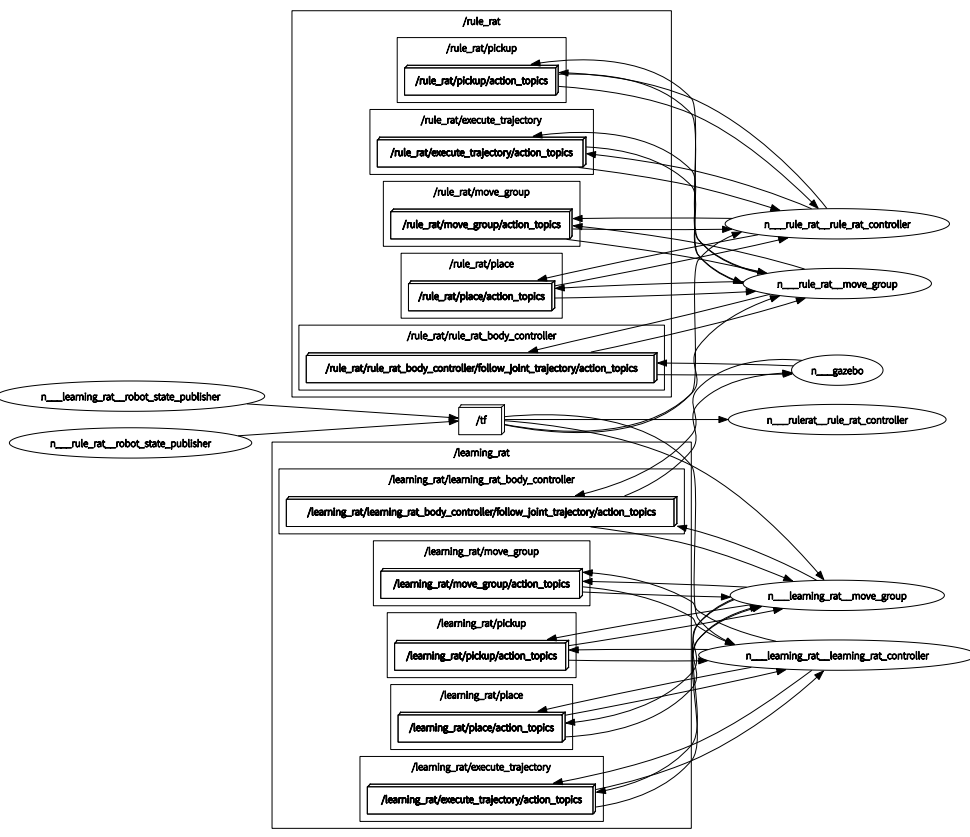
\includegraphics[width=0.95\linewidth]{images/appendix/rosgraph.png}
  \caption{仿真平台节点}\label{figure_rosgraph}
\end{figure}


\newpage
\section{Controller List}\label{appendix_controllerlist}
\begin{table}[htb]
  \linespread{1.5}
  \zihao{5}
  \centering
  \caption{ros\_control中Controller List}\label{table_controllerlist}
  \begin{tabular}{p{6.5cm}<{\centering\arraybackslash}p{3.5cm}<{\centering\arraybackslash}}
    \toprule
    Controller &  控制器类型  \\ \midrule
    $left\_wheel\_velocity\_controller$         & 速度控制器 \\
    $right\_wheel\_velocity\_controller$        & 速度控制器 \\
    $base\_to\_body\_link1\_joint\_controller$  & 位置控制器 \\
    $body\_link1\_to\_link2\_joint\_controller$ & 位置控制器 \\
    $body\_link2\_to\_link3\_joint\_controller$ & 位置控制器 \\
    $body\_link3\_to\_link4\_joint\_controller$ & 位置控制器 \\
    $body\_link4\_to\_link5\_joint\_controller$ & 位置控制器 \\
    $body\_link5\_to\_link6\_joint\_controller$ & 位置控制器 \\
    $body\_link6\_to\_head\_joint\_controller$  & 位置控制器 \\
    $joint\_state\_controller$                  & 状态控制器 \\
    \bottomrule
    \end{tabular}
\end{table}

